
\section{The qubit}
The quantum bit, the qubit, is the building block of quantum computing.
Like the classical binary digit it can be either 0 or 1.
But being quantum, these are quantum states, $\ket{0}$ and $\ket{1}$, and the qubit can be in any superposition of these states.
The state of the qubit lies in a two-dimensional Hilbert space, and the states $\ket{0}$ and $\ket{1}$ are basis vectors, known as the computational basis states.
Thus, the state of a qubit can be expressed as
\begin{equation}
    \ket{\psi} = \alpha \ket{0} + \beta \ket{1} = \begin{pmatrix} \alpha \\ \beta \end{pmatrix}
    \label{eq:qubit}
\end{equation}
where $\alpha$ and $\beta$ are any numbers, even complex ones.
The only requirement is that the state is normalised, i.e., $\vert\alpha\vert^2 + \vert\beta\vert^2 = 1$.

Normalisation is required due to the Born rule, as the absolute square of the coefficients is the probability of measuring the qubit in the corresponding basis state.
It is one of nature's great mysteries what exactly a measurement is, but in the quantum computational setting, it can be thought of as taking a random sample with the probabilities given by the coefficients, which can be done systematically.

\subsection{The Bloch sphere}
A useful tool for visualising the state of a qubit is the Bloch sphere.
First, it should be noted for states on the form \cref{eq:qubit} are not unique, only the relative complex phase matters.
There is a global phase which is not measurable, and thus not relevant for the state of the qubit.
Therefore, taking also the normalisation requirement into account, the state of the qubit can be expressed as
\begin{equation}
    \ket{\psi} = \cos\left(\frac{\theta}{2}\right) \ket{0} + e^{i\phi} \sin\left(\frac{\theta}{2}\right) \ket{1}
    \label{eq:bloch}
\end{equation}
where $\theta, \phi \in \mathbb{R}$.
Interpreting $\theta$ as the polar angle and $\phi$ the azimuthal angle, the state of the qubit can be identified with a point a sphere, the Bloch sphere.
There, the state $\ket{0}$ is typically thought of as the north pole, and $\ket{1}$ as the south pole.
\Cref{fig:bloch} shows the Bloch sphere with the state of the qubit in \cref{eq:bloch}.

\begin{figure}
    \centering
    \def\svgwidth{0.4\textwidth}
    %% Creator: Inkscape 1.2.1 (9c6d41e, 2022-07-14), www.inkscape.org
%% PDF/EPS/PS + LaTeX output extension by Johan Engelen, 2010
%% Accompanies image file 'bloch_sphere.pdf' (pdf, eps, ps)
%%
%% To include the image in your LaTeX document, write
%%   \input{<filename>.pdf_tex}
%%  instead of
%%   \includegraphics{<filename>.pdf}
%% To scale the image, write
%%   \def\svgwidth{<desired width>}
%%   \input{<filename>.pdf_tex}
%%  instead of
%%   \includegraphics[width=<desired width>]{<filename>.pdf}
%%
%% Images with a different path to the parent latex file can
%% be accessed with the `import' package (which may need to be
%% installed) using
%%   \usepackage{import}
%% in the preamble, and then including the image with
%%   \import{<path to file>}{<filename>.pdf_tex}
%% Alternatively, one can specify
%%   \graphicspath{{<path to file>/}}
%% 
%% For more information, please see info/svg-inkscape on CTAN:
%%   http://tug.ctan.org/tex-archive/info/svg-inkscape
%%
\begingroup%
\makeatletter%
\providecommand\color[2][]{%
  \errmessage{(Inkscape) Color is used for the text in Inkscape, but the package 'color.sty' is not loaded}%
  \renewcommand\color[2][]{}%
}%
\providecommand\transparent[1]{%
  \errmessage{(Inkscape) Transparency is used (non-zero) for the text in Inkscape, but the package 'transparent.sty' is not loaded}%
  \renewcommand\transparent[1]{}%
}%
\providecommand\rotatebox[2]{#2}%
\newcommand*\fsize{\dimexpr\f@size pt\relax}%
\newcommand*\lineheight[1]{\fontsize{\fsize}{#1\fsize}\selectfont}%
\ifx\svgwidth\undefined%
  \setlength{\unitlength}{177.93310547bp}%
  \ifx\svgscale\undefined%
    \relax%
  \else%
    \setlength{\unitlength}{\unitlength * \real{\svgscale}}%
  \fi%
\else%
  \setlength{\unitlength}{\svgwidth}%
\fi%
\global\let\svgwidth\undefined%
\global\let\svgscale\undefined%
\makeatother%
\begin{picture}(1,1.06027363)%
  \lineheight{1}%
  \setlength\tabcolsep{0pt}%
  \put(0,0){\includegraphics[width=\unitlength,page=1]{bloch_sphere.pdf}}%
  \put(0.2887321,0.28921972){\color[rgb]{0,0,0}\makebox(0,0)[lt]{\lineheight{0}\smash{\begin{tabular}[t]{l}$x$\\ \end{tabular}}}}%
  \put(0.97157299,0.44096214){\color[rgb]{0,0,0}\makebox(0,0)[lt]{\lineheight{0}\smash{\begin{tabular}[t]{l}$y$\end{tabular}}}}%
  \put(0.45522726,0.9935414){\color[rgb]{0,0,0}\makebox(0,0)[lt]{\lineheight{0}\smash{\begin{tabular}[t]{l}$z$\end{tabular}}}}%
  %\put(0.44047452,0.41690636){\color[rgb]{0,0,0}\makebox(0,0)[lt]{\lineheight{0}\smash{\begin{tabular}[t]{l}φ\end{tabular}}}}%
  \put(0.44047452,0.41690636){\color[rgb]{0,0,0}\makebox(0,0)[lt]{\lineheight{0}\smash{\begin{tabular}[t]{l}$\phi$\end{tabular}}}}%
  % \put(0.45101219,0.69597371){\color[rgb]{0,0,0}\makebox(0,0)[lt]{\lineheight{0}\smash{\begin{tabular}[t]{l}θ\end{tabular}}}}%
  \put(0.45101219,0.69597371){\color[rgb]{0,0,0}\makebox(0,0)[lt]{\lineheight{0}\smash{\begin{tabular}[t]{l}$\theta$\end{tabular}}}}%
  \put(0,0){\includegraphics[width=\unitlength,page=2]{bloch_sphere.pdf}}%
  \put(0.04935377,0.94994952){\color[rgb]{0,0,0}\makebox(0,0)[lt]{\lineheight{0}\smash{\begin{tabular}[t]{l} \end{tabular}}}}%
  % \put(0,0){\includegraphics[width=\unitlength,page=3]{figs/bloch/bloch_sphere.pdf}}%
  \put(0.46622932,0.0080449){\color[rgb]{0,0,0}\makebox(0,0)[lt]{\lineheight{0}\smash{\begin{tabular}[t]{l}$\ket{1}$\end{tabular}}}}%
  % \put(0,0){\includegraphics[width=\unitlength,page=4]{figs/bloch/bloch_sphere.pdf}}%
  \put(0.35242254,0.95312728){\color[rgb]{0,0,0}\makebox(0,0)[lt]{\lineheight{0}\smash{\begin{tabular}[t]{l}$\ket{0}$\end{tabular}}}}%
  % \put(0,0){\includegraphics[width=\unitlength,page=5]{figs/bloch/bloch_sphere.pdf}}%
  % \put(0.6104334,0.7732887){\color[rgb]{0,0,0}\makebox(0,0)[lt]{\lineheight{0}\smash{\begin{tabular}[t]{l}ψ\end{tabular}}}}%
  \put(0.6104334,0.7732887){\color[rgb]{0,0,0}\makebox(0,0)[lt]{\lineheight{0}\smash{\begin{tabular}[t]{l}$\ket{\psi}$\end{tabular}}}}%
\end{picture}%
\endgroup%

    \caption{
        The Bloch sphere in which a qubit state is represented by a point.
        The state $\ket{0}$ is the north pole, and $\ket{1}$ is the south pole.
        The latitudinal angle $\theta$ determines the probability of measuring the qubit in the state $\ket{0}$, while the longitudinal angle $\phi$ corresponds to the complex phase.
        From \cite{wikipedia_bloch}.
    }
    \label{fig:bloch}
\end{figure}

\subsection{Multiple qubits}
Although the continuous nature of the qubit is indeed useful, the true power of quantum computers lie in how multiple qubits interact.
Having multiple qubits allows for the creation of entanglement, which is a key feature of quantum computing.

With just two qubits, there are four possible states, $\ket{00}, \ket{01}, \ket{10}, \ket{11}$.
Each of these four have their own probability amplitude, and thus their own probability of being measured.
A two-qubit system will therefore operate on with four complex numbers.

Generally, the state of multiple qubits can be expressed using the tensor product as
\begin{equation}
    \ket{\psi_1 \psi_2 \cdots  \psi_n} = \ket{\psi_1} \otimes \ket{\psi_2} \otimes \cdots \otimes \ket{\psi_n}
    \label{eq:tensor}.
\end{equation}
What makes this so powerful is that the state of a multi-qubit system can be anything on the form
\begin{equation}
    \ket{\psi_1 \psi_2 \cdots  \psi_n}
    = c_1 \ket{0\dots 00} + c_2 \ket{0\dots 01} + \cdots + c_{2^n} \ket{1\dots 11}
    = \begin{pmatrix}
        c_1 \\ c_2 \\ \vdots \\ c_{2^n}
    \end{pmatrix}
    \in \mathbb{C}^{2^n},
    \label{eq:superposition}
\end{equation}
which means that with $n$ qubits, the system can be in any superposition of the $2^n$ basis states.
Operating on several qubits then, one can do linear algebra in an exponentially large space.